% Cloud Job-Processing Service -- design report (max 5 pages incl. diagrams)
% Build: latexmk -pdf main.tex   (or upload report/ + diagrams/ to Overleaf)
\documentclass[10pt,a4paper]{article}
\usepackage[margin=1.6cm,top=1.4cm,bottom=1.5cm]{geometry}
\usepackage[T1]{fontenc}
\usepackage{lmodern}
\usepackage{microtype}
\usepackage{graphicx}
\usepackage{booktabs}
\usepackage{tabularx}
\usepackage{enumitem}
\usepackage{xcolor}
\usepackage[hidelinks]{hyperref}
\usepackage{titlesec}
\usepackage{float}
\setlist{nosep,leftmargin=*}
\setlength{\parskip}{2.5pt}
\setlength{\parindent}{0pt}
\titlespacing*{\section}{0pt}{6pt}{2pt}
\titleformat*{\section}{\large\bfseries}
\titlespacing*{\subsection}{0pt}{4pt}{1pt}
\titleformat*{\subsection}{\normalsize\bfseries}
\newcolumntype{Y}{>{\raggedright\arraybackslash}X}
\renewcommand{\arraystretch}{1.08}

\begin{document}
\begin{center}
{\Large\bfseries Multi-Cloud Wildlife-Image Job-Processing Service: Design}\\[2pt]
Lucas Huang
\end{center}
\vspace{-6pt}

% =====================================================================
\section{Overview, Assumptions and Key Decisions}
Partners upload a 1--5\,GB image batch; each job runs \emph{prep} (CPU) $\rightarrow$
\emph{species ID} (GPU) $\rightarrow$ \emph{report} (CPU). The design rests on three ideas:
(i)~one transactional store (PostgreSQL) holds job state, the queue and leases, so there is never a
dual-write between a queue and a database;
(ii)~workers \emph{pull} leases carrying a monotonically increasing \emph{fencing epoch}, and outputs
are written to per-attempt immutable prefixes and published by a conditional update,
so a result is published exactly once even if a worker reappears;
(iii)~\emph{compute is active-active across AWS and GCP, state is active-passive}, and every job is
processed \emph{data-locally} in its home cloud to avoid egress.

\begin{table}[H]\centering\small
\begin{tabularx}{\linewidth}{@{}p{3.1cm}Y@{}}
\toprule
\textbf{Assumption} & \textbf{Value and consequence} \\ \midrule
Workload & 100 jobs/day; burst 100/h; mean batch 3\,GB ($\approx$1{,}000 JPEGs); mean job 15\,min split
  5/6/4\,min (prep/ID/report); prep output $\approx$5--10\% of input (resized images). \\
GPU is the bottleneck & 4 GPUs $\times$ 60/6 = \textbf{40 jobs/h}. A 100-job burst drains in \textbf{2.5\,h}
  (worst case, all 30-min jobs: 5\,h) $\Rightarrow$ durable queue, ETA shown to users, acceptance never
  blocks on capacity. Daily GPU use is 10 of 96 GPU-h ($\approx$10\%) $\Rightarrow$ GPU pools scale 0--2 per cloud. \\
CPU sizing & Burst prep 100$\times$5\,min $\approx$ 9 VMs; report is GPU-bound (40$\times$4\,min $\approx$ 3 VMs)
  $\Rightarrow$ $\approx$12 of 16 CPU VMs at peak. \\
VM cap & Worker VMs only: per cloud 0--2 GPU + 1--8 CPU = \textbf{10 per cloud, 20 total}. The control
  plane (API, DB, storage, K8s masters) is managed/serverless. If it must count, 1 VM per cloud is
  carved out, leaving 18 workers, which still covers peak demand. \\
Network & Partner $\rightarrow$ storage burst 300\,GB/h $\approx$ 670\,Mbps aggregate (direct multipart
  upload, not via the API). VM $\leftrightarrow$ object store $\geq$5\,Gbps. AWS$\leftrightarrow$GCP HA VPN
  (4 tunnels $\times$ 1.25\,Gbps) $\approx$2.5\,Gbps usable, same-metro RTT $<$5\,ms. \\
Pricing (indicative) & Egress $\approx$\$0.12/GB; GPU VM $\approx$\$1.2/h; standard object storage
  $\approx$\$0.025/GB-month. Always-on 4 GPUs $\approx$\$3.5k/month vs.\ scale-to-demand
  ($\approx$10 GPU-h/day + 1 warm GPU in business hours) $\approx$\$0.8k/month, at the cost of a
  $\approx$5\,min cold start. \\
Regions & Both clouds in Sydney: widest Australian GPU supply; data stays in Australia
  (camera traps can capture people, so images may be personal information). \\
Third parties & Partner OIDC IdP; provider-neutral DNS with health checks; a small serverless
  witness for DB leadership; GitHub Actions. Supplied programs are CLI tools (input dir $\rightarrow$
  output dir, exit code); model weights ($\approx$1\,GB) are kept in our own buckets, so nothing is
  pulled from public hubs at run time. \\
\bottomrule
\end{tabularx}
\end{table}
\vspace{-8pt}

\begin{figure}[H]\centering
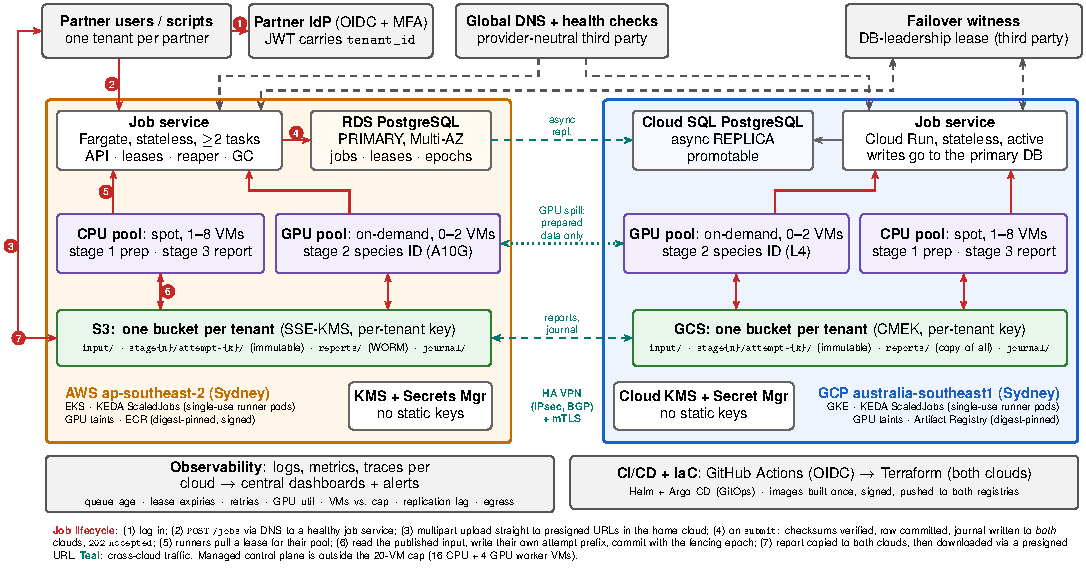
\includegraphics[width=\linewidth]{../diagrams/architecture.pdf}
\vspace{-14pt}
\caption{Architecture. Red numbers follow one job; teal links are the only cross-cloud traffic.}
\label{fig:arch}
\end{figure}
\vspace{-10pt}

% =====================================================================
\section{One Job's Lifecycle}
\textbf{States:} \texttt{UPLOADING} $\rightarrow$ \texttt{ACCEPTED} $\rightarrow$
for each stage \texttt{QUEUED} $\rightarrow$ \texttt{RUNNING} $\rightarrow$ \texttt{SUCCEEDED}
$\rightarrow$ \texttt{COMPLETED}; side exits \texttt{FAILED\_NEEDS\_REVIEW}, \texttt{CANCELLED}.
(1)~The partner logs in through its IdP and gets a JWT carrying \texttt{tenant\_id}.
(2)~\texttt{POST /jobs} (file list, sizes, SHA-256) reaches a healthy job service. The job service picks
the \emph{home cloud} (healthy, lowest estimated wait) and returns presigned multipart-upload URLs
scoped to \texttt{jobs/\{id\}/input/} in the tenant bucket (15\,min).
(3)~The client uploads directly; failed parts are retried individually.
(4)~\texttt{POST /jobs/\{id\}:submit} (with an \texttt{Idempotency-Key}) verifies checksums, commits
\texttt{ACCEPTED} + \texttt{PREP\_QUEUED}, writes a small acceptance record to \emph{both} clouds' journals,
and only then returns \texttt{202} with the job ID.
(5)~A CPU runner in the home cloud claims the prep lease;
(6)~it reads the input, writes \texttt{stage1/attempt-k/} and commits. That commit queues the GPU stage in
the same transaction, and stage 3 follows the same way.
(7)~The report is copied to both clouds; only then is the job \texttt{COMPLETED}. A notification
(transactional outbox) is sent, and \texttt{GET /jobs/\{id\}/report} returns a 5-minute presigned URL.
\texttt{GET /jobs/\{id\}} shows the stage, queue position and ETA at any time.

% =====================================================================
\section{Job Coordination and Placement}
\textbf{Acceptance and tracking.} The \texttt{jobs} and \texttt{stage\_runs} tables are the single source of
truth. Each stage row holds \texttt{status}, \texttt{epoch}, \texttt{lease\_owner},
\texttt{lease\_expires\_at} (database clock only, never worker clocks) and \texttt{published\_attempt}.
Load is $<$1\,write/s, far below PostgreSQL limits, so a separate broker (SQS/PubSub) would add a
dual-write hazard without benefit.

\textbf{Worker discovery and assignment (pull).} A small \emph{runner agent} is baked into each stage image.
It calls \texttt{POST /leases} with its capabilities (\texttt{cloud}, \texttt{stage}, \texttt{gpu},
\texttt{mem\_gb}). The coordinator selects a row with \texttt{SELECT \ldots FOR UPDATE SKIP LOCKED} and,
in the same transaction, sets \texttt{RUNNING}, increments \texttt{epoch}, and sets the lease to 90\,s.
It returns \texttt{(job, stage, attempt, epoch)} plus credentials scoped to that job (\S\ref{sec:sec}).
Workers therefore need no registry: a worker exists while it is renewing leases, and VMs that never ask
receive no work. Pull also balances load naturally, because idle runners take the next item.

\textbf{Stage dependencies.} A stage becomes \texttt{QUEUED} only inside the transaction that publishes
its predecessor; downstream stages read only the \emph{published} attempt pointer, never a prefix
listing.

\textbf{Resources and placement.} At submission each job gets a size class (S/M/L by batch size), which
maps to a memory requirement. A lease matches only if the runner's pool satisfies it: GPU stages run only
on tainted GPU pools, and L-class prep runs on the 32\,GB node group. Ordering is \emph{weighted fair
share across tenants}, then oldest first, with a per-tenant cap of 2 concurrent GPU stages, so one
partner's 50-job burst cannot starve the others.
\textbf{Data-local placement:} prep runs in the home cloud. The GPU stage \emph{spills} to the other
cloud only if $\mathrm{ETA}_{home} > \mathrm{ETA}_{other} + t_{transfer} + 20\,\mathrm{min}$ (hysteresis);
it then moves the \emph{prepared} output ($\approx$150\,MB, $\approx$\$0.02) rather than the raw
3\,GB batch ($\approx$\$0.36). The report stage has small inputs and runs on whichever cloud has a free
CPU runner.

% =====================================================================
\section{VMs, Containers and Orchestration}
\textbf{Provisioning (IaC).} Terraform modules per cloud (VPC, HA VPN, EKS/GKE, node pools, buckets with
lifecycle rules, KMS, databases, IAM) plus a global stack (DNS, witness). State lives in an encrypted
remote backend with locking. GitHub Actions runs \texttt{plan} on pull requests and \texttt{apply} after
review, authenticating with OIDC federation (no cloud keys in CI). In-cluster objects are Helm charts
synced by Argo CD (GitOps), so both clouds run identical, versioned manifests. Node pools enforce the cap
in IaC (\texttt{max\_size}: GPU 2, CPU 8 per cloud), and an alert fires if the VM count reaches 19.
Spot is used for CPU (a preemption is just another lease expiry); GPU is on-demand (scarce, only 4
slots).

\textbf{Containers.} There is one image per stage: the supplied program + the runner agent, built once
in CI, scanned, signed (cosign), pushed to both registries and deployed \emph{by digest}. The GPU image
pins the CUDA base, framework versions and driver range. Model weights are \emph{not} baked in (the same
pattern as my A1 SmartPark deployment): an init container fetches \texttt{model@version} from our bucket,
verifies its SHA-256, and stores it in a node-local read-only cache, so restarts do not re-download it.

\textbf{Isolation and scaling.} KEDA \emph{ScaledJobs} create one single-use pod per queued lease
(trigger: queued count for that stage and cloud, from the coordinator's metrics endpoint). Each pod runs
exactly one attempt and exits, so every tenant job gets a fresh filesystem. Pod requests ($\approx$90\%
of a node) place one stage per VM. The cluster autoscaler adds and removes nodes within the pool bounds;
GPU pools scale to zero after 10\,min idle, except one warm GPU in business hours. Pods run as non-root
with a read-only root filesystem, all capabilities dropped and seccomp \texttt{RuntimeDefault}.
NetworkPolicy is default-deny; the only egress allowed is to the coordinator and private storage
endpoints, so a third-party program cannot exfiltrate data.

% =====================================================================
\section{Storage and ML Reproducibility}
\begin{table}[H]\centering\small
\begin{tabularx}{\linewidth}{@{}p{2.3cm}p{3.6cm}Y@{}}
\toprule
\textbf{Data} & \textbf{Store} & \textbf{Durability, lifecycle and cleanup} \\ \midrule
Inputs & S3/GCS, bucket per tenant, home cloud & Object stores are designed for 11 nines; versioned. Deleted 30\,days after the job
  ends (partners keep originals). Not replicated cross-cloud (9\,TB/month would cost $\approx$\$1{,}080/month in egress). \\
Intermediates & same bucket, \texttt{stage\{n\}/attempt-\{k\}/} & Immutable, \texttt{\_MANIFEST.json} (files + SHA-256) written \emph{last}.
  Unpublished attempts are GC'd after 24\,h; published ones 7\,days after the job ends. \\
Reports & both clouds, \texttt{reports/} & Versioning + object lock (WORM, 1\,year); copied to the second cloud \emph{before} \texttt{COMPLETED}
  (RPO\,=\,0); Infrequent Access tier after 30\,days. \\
Metadata & RDS PostgreSQL (Multi-AZ) $\rightarrow$ Cloud SQL replica & PITR 14\,days, daily snapshot, async logical replica in GCP
  (lag typically $<$5\,s). Acceptance journal in both clouds closes the lag gap. \\
\bottomrule
\end{tabularx}
\end{table}
\vspace{-6pt}
\textbf{Provenance.} Each published stage run stores an immutable record: input-manifest hash, image
digest, program version, model name/version/SHA-256, framework/CUDA/driver versions, instance type,
cloud/region, attempt, epoch, timings, exit code and output-manifest hash. The report embeds a
provenance digest, so a result can be re-run with exactly the same artefacts. Images and model versions
referenced by retained reports are exempt from registry clean-up.

% =====================================================================
\section{Health and Recovery}
\textbf{Readiness.} The GPU pod's startup probe passes only after the model is loaded, a CUDA self-test
succeeds and storage is reachable. A runner claims leases only when ready. The node health is taken from
the kubelet and the GPU device plugin (Xid errors).
\textbf{Crashes.} A non-zero exit or OOM is reported as a \emph{program failure}. A lost pod, VM,
preemption or partition shows up as missing heartbeats (every 30\,s); the reaper expires the lease after
90\,s, increments the epoch and requeues the stage on another node.
\textbf{Stalls.} Heartbeats carry progress (child CPU time, bytes written). If progress is unchanged for
10\,min, or a per-stage deadline of 2$\times$ the historical p99 for the size class is exceeded, the
attempt is killed and requeued. The agent also \emph{self-fences}: if it cannot renew its lease, it stops
the program before the lease expires and writes nothing more.

\textbf{Repeated failures.} Infrastructure failures do not consume the job's retry budget; they lower the
\emph{node's} health score, and 2 failures from different jobs within 1\,h cordon and replace that node.
Program failures are retried at most twice with exponential backoff; after an OOM, the retry goes to the
next memory class. After that the job becomes \texttt{FAILED\_NEEDS\_REVIEW} (poison job): the input is
kept, the partner and operator are notified, and the queue continues.

\textbf{Logs and metrics.} Structured JSON logs carry \texttt{job\_id, tenant\_id, stage, attempt, epoch,
node, image digest, model hash}, and an OpenTelemetry trace spans the three stages. Alerts: oldest queued
age $>$3\,h, lease expiries/h, retry rate, stage p50/p99 by size class, GPU utilisation and memory, VM
count vs.\ cap, DB replication lag $>$60\,s, egress bytes/day, per-tenant failure rate.

% =====================================================================
\section{Failure Scenario: GPU VM Lost After Writing Its Output}
\begin{table}[H]\centering\small
\begin{tabularx}{\linewidth}{@{}p{1.25cm}Y@{}}
\toprule
\textbf{Time} & \textbf{Event and state change} \\ \midrule
$t_0$ & G1 holds the stage-2 lease of job J with \texttt{epoch=7}; it writes \texttt{stage2/attempt-7/} and then \texttt{\_MANIFEST.json}. \\
$t_1$ & G1 becomes unreachable before \texttt{commit}; its heartbeats stop. Its scoped credentials expire with the lease. \\
$t_1$+90\,s & The reaper, in one transaction, sets \texttt{epoch=8}, attempt 7 \texttt{ABANDONED}, stage \texttt{QUEUED}.
  \emph{Optimisation:} if attempt 7's manifest exists and every checksum verifies, the reaper \emph{adopts} it and
  publishes attempt 7 under \texttt{epoch=8} (saves $\approx$6 GPU-min); otherwise G2 claims the lease. \\
$t_2$ & G2 writes \texttt{stage2/attempt-8/} and commits:
  \texttt{UPDATE stage\_runs SET status='SUCCEEDED', published\_attempt=8 WHERE job=J AND stage=2 AND epoch=8 AND status='RUNNING'}
  $\rightarrow$ 1 row; stage 3 is queued in the same transaction. \\
$t_3$ & G1 returns and commits with \texttt{epoch=7} $\rightarrow$ 0 rows $\rightarrow$ \texttt{409 STALE\_EPOCH}. The agent discards
  its work and exits. Kubernetes has already deleted the pod, so the kubelet kills it on reconnect. \\
$t_3$+24\,h & GC deletes the unpublished \texttt{attempt-7/} prefix. \\
\bottomrule
\end{tabularx}
\end{table}
\vspace{-6pt}
\textbf{Why there is no duplicate or conflicting result:} (a)~attempts never share a path, so G1 cannot
overwrite G2; (b)~exactly one attempt per stage can satisfy the epoch predicate; (c)~consumers follow the
published pointer only, so an orphan is invisible; (d)~the report pointer and the outbox notification are
written in the same transaction as \texttt{COMPLETED}, so a stale worker can never trigger a second
report or e-mail; (e)~the lease clock is the database clock, so G1's clock drift cannot help it.

% =====================================================================
\section{Multi-Cloud Operation}
\textbf{Strategy: active-active compute, active-passive state (warm standby).} Both clouds run job
services and workers every day, so failover capacity is always warm and tested. The only singleton is
the database writer (AWS); GCP holds an async replica that can be promoted. A fully active-active
multi-master DB (e.g.\ CockroachDB) would need $\geq$3 regions for quorum and a third-party dependency,
which is too much for 100 jobs/day.

\textbf{Connectivity and data movement.} An AWS Site-to-Site VPN $\leftrightarrow$ GCP HA VPN link (4 IPsec
tunnels, BGP, non-overlapping CIDRs) carries control traffic with mTLS on top. Over it go: DB logical
replication; GCP job-service writes to the primary DB; report and journal copies; and rare GPU spills.
Bulk inputs never cross. Cross-cloud reads use short-lived presigned URLs, so no long-lived cross-cloud
IAM trust is needed. \textbf{Egress:} data-local placement cuts cross-cloud bytes from $\approx$9\,TB/month
($\approx$\$1{,}080) to $\approx$30\,GB/month ($\approx$\$4). A dedicated interconnect is not justified
at this volume.

\textbf{Dynamic failover (AWS unreachable).}
(1)~\emph{Detection:} external DNS health checks from several locations, plus GCP probes, fail for 3\,min.
(2)~\emph{No split-brain:} the AWS coordinator must renew a 60\,s leadership lease in the witness. If it
cannot, it stops granting leases and accepting writes. GCP waits 2$\times$ that lease before promoting
Cloud SQL and increments a \emph{control-plane generation}; every request carries the generation, so a
reconnecting old primary is refused.
(3)~DNS sends all API traffic to GCP; the GCP coordinator replays both journals, re-creating any accepted
job lost to replication lag (RPO\,=\,0 for accepted jobs), and extends all running GCP leases by one grace
period. Workers retry buffered commits with idempotency keys.
\emph{Keeps operating:} new submissions (homed in GCP), all GCP-homed jobs, status for every job, and
download of every report. \emph{Paused, not lost:} AWS-homed jobs whose inputs are in S3; they resume
when AWS returns. Capacity drops to 10 VMs (20 jobs/h on GPU), because the unreachable cloud's VMs might
still be running and must still count against the cap. RTO $\approx$5\,min.
\textbf{Failback:} the old AWS database is rebuilt as a replica of GCP, then switched back in a quiet
window. A GCP outage is simpler: AWS stays primary and only GCP-homed jobs pause.

% =====================================================================
\section{Cloud Security}\label{sec:sec}
\textbf{Users.} Partners sign in through OIDC with MFA (their own IdP federated, or our user pool) and
receive 1\,h JWTs carrying \texttt{tenant\_id} and a role (submitter/viewer/admin). Automation uses OAuth
client credentials per partner.
\textbf{Services.} Workloads use workload identity (EKS Pod Identity, GKE Workload Identity), so no
static cloud keys exist anywhere. Service-to-service calls use mTLS with SPIFFE-style identities, and
the few cross-cloud API calls use workload-identity federation.

\textbf{Access control (defence in depth).}
(1)~The API derives the tenant from the token, never from the request body.
(2)~PostgreSQL row-level security on \texttt{tenant\_id} (\texttt{SET app.tenant\_id} per transaction).
(3)~One bucket and one KMS key per tenant per cloud.
(4)~Per-lease credentials minted via STS session policies / GCP credential access boundaries: read
\texttt{input/} and the published predecessor, write only this attempt's prefix, TTL\,=\,lease.
(5)~Presigned URLs are per object and short-lived.
Deleting a tenant's key crypto-shreds its data when the partnership ends.

\textbf{Secrets.} Secrets live in AWS Secrets Manager / GCP Secret Manager, read at run time through
workload identity and rotated every 30\,days. DB access uses IAM authentication. Secret scanning runs in
CI; images contain no secrets.
\textbf{Network isolation.} Workers sit in private subnets without public IPs and reach storage through
private endpoints (S3 gateway endpoint, Private Google Access). Databases have no public endpoint. The
API sits behind a WAF and rate limits, and admission control (Kyverno / Binary Authorization) admits
only signed images.
\textbf{Encryption.} TLS 1.2+ externally, mTLS internally, and IPsec between clouds (two layers). At rest:
SSE-KMS/CMEK with per-tenant keys for objects, KMS-encrypted DB, disks and backups. Audit trail:
CloudTrail data events, GCS data-access logs, and DB audit of all state transitions.

% =====================================================================
\section{Trade-offs and Limitations}
Async DB replication trades a few seconds of metadata RPO for write latency (the journal compensates).
Not replicating inputs saves $\approx$\$1k/month but pauses home-cloud jobs during an outage. Scale-to-zero
GPUs save $\approx$\$2.7k/month for a $\approx$5\,min cold start. The witness and DNS are third-party
dependencies: if both fail, failover becomes a manual, operator-approved promotion.

\end{document}
